\documentclass[11pt,letterpaper]{article}
\usepackage[margin=1in]{geometry}
\usepackage{amsmath,amssymb,graphicx,booktabs,setspace,caption,hyperref}
\onehalfspacing
\widowpenalty=10000
\clubpenalty=10000
\renewcommand{\topfraction}{0.9}
\renewcommand{\textfraction}{0.08}
\renewcommand{\floatpagefraction}{0.85}
\graphicspath{{../results/figures/}}
\hypersetup{hidelinks,pdftitle={Modeling and Controlled Validation of a Pan-Tilt Camera}}
% Replace the author field before submission. Course confirmed by the user.
\newcommand{\ReportAuthor}{\textit{Author name to be entered}}
\newcommand{\ReportCourse}{ECE 5240 Robot Perception}

% Generated by run.py from results/summary.json; do not edit.
\newcommand{\HeightAreaMin}{34.56}
\newcommand{\HeightAreaMax}{311.04}
\newcommand{\HeightAreaError}{2.06\times 10^{-16}}
\newcommand{\PanAreaError}{4.12\times 10^{-16}}
\newcommand{\TiltAreaFirst}{10373.87}
\newcommand{\TiltAreaLast}{140.60}
\newcommand{\EntryTime}{0.9282}
\newcommand{\ExitTime}{11.0718}
\newcommand{\FirstSampleTime}{0.94}
\newcommand{\LastSampleTime}{11.06}
\newcommand{\ImageSpeed}{3.5490}
\newcommand{\VisibleSamples}{507}
\newcommand{\MotionSamples}{601}
\newcommand{\CriticalHeight}{2.8}
\newcommand{\NoiseError}{0.000640}
\newcommand{\NoisePercentError}{0.905}
\newcommand{\NoiseMaxRMSE}{0.706817}
\newcommand{\JacobianFirst}{5.74\times 10^{-9}}
\newcommand{\JacobianLast}{1.02\times 10^{-13}}

\title{Modeling and Controlled Validation\\of a Pan-Tilt Camera}
\author{\ReportAuthor\\\ReportCourse\\Instructor: Silvia Ferrari}
\date{}
\begin{document}
\begin{titlepage}
\maketitle
\thispagestyle{empty}
\vfill
\begin{center}Midterm Project Technical Report\\
Source code, configuration, numerical data, and media accompany this report.
\end{center}
\vfill
\end{titlepage}

\begin{abstract}
A virtual pan-tilt (PT) camera is developed to examine how sensor position, orientation, target motion, and environmental occlusion affect image-position measurements and field-of-view (FOV). An ideal pinhole model is combined with positive-depth selection, solid-box line-of-sight testing, and optional Gaussian measurement noise. Controlled experiments vary one factor at a time, while a three-dimensional animation illustrates combined motion. Increasing nadir-view height from 4 to 12 m increases coverage from \HeightAreaMin{} to \HeightAreaMax{} m$^2$, consistent with quadratic scaling. Analytic and simulated visibility agree at every sampled time in a moving-target experiment and at every sampled obstacle height, including the 2.8 m grazing threshold. Projection derivatives agree with central differences, and Monte Carlo radial error follows the assumed noise model. These results verify selected properties of the synthetic sensor; they do not establish physical-camera accuracy.
\end{abstract}

\section{Introduction}
The project specification calls for a mathematical sensor model, measurement and FOV simulation, and evidence of dependencies on sensor pose, targets, and the environment\cite{assignment}. A PT camera is appropriate because its orientation changes image coordinates and the visible portion of a workspace. The course handout supplies the pinhole geometry and a broader position--velocity measurement model\cite{handout}. This project adopts its position-measurement component and extends visibility with occlusion and noise.

The objective is to verify five predictions: coverage changes with height; pan and tilt have different geometric effects; a moving target crosses the image boundary at predictable times; an obstacle can suppress an otherwise valid observation; and the assumed noise produces a known radial RMS. A numerical sensitivity check supports the graduate-level mathematical analysis. Prescribed poses are sufficient for these sensor questions; no feedback controller or motor model is claimed. The report follows the technical-report organization and formatting guidance\cite{writing}.

\section{Theory and Methods}
\subsection{Coordinates and pinhole measurement}
World $Z=0$ is a horizontal ground plane. The camera center is $C$ and a ground target is $X=[x,y,0]^T$. The camera frame is right-handed, with its $z$ axis along the optical axis. Define the camera-to-world rotation using right-handed active rotations:
\begin{equation}
R=R_z(\psi)R_x(\phi),\qquad q=R^T(X-C).
\label{eq:pose}
\end{equation}
Pan $\psi$ rotates about world $Z$; tilt $\phi$ rotates about the intermediate $x$ axis. Thus $R^T=R_x^TR_z^T$, equivalent to the product of the handout's passive matrices $R_\phi R_\psi$. This convention prevents ambiguity between active rotations and coordinate transformations. At $\phi=180^\circ$ the optical axis points downward; at $\psi=0$, $\phi=140^\circ$ it points downward and toward negative world $Y$.

Similar triangles on a virtual image plane at focal length $f$ give
\begin{equation}
p=\pi(q)=f\begin{bmatrix}q_x/q_z\\q_y/q_z\end{bmatrix},\qquad q_z>0.
\label{eq:projection}
\end{equation}
Image coordinates are physical lengths; plots convert meters to millimeters. They are not pixels. For image width $a$ and height $b$, geometric FOV membership requires
\begin{equation}
q_z>0,\qquad |p_x|\leq a/2,\qquad |p_y|\leq b/2.
\label{eq:fov}
\end{equation}
Positive depth is essential: a point behind the camera is unavailable even if its formal projection lies inside the rectangle.

\subsection{Ground footprint and geometric predictions}
For each image corner, $d_i^C=[\pm a/2,\pm b/2,f]^T$ and $d_i^W=Rd_i^C$. Its ground intersection is
\begin{equation}
P_i=C+t_i d_i^W,\qquad t_i=-C_z/(d_i^W)_z.
\label{eq:ray}
\end{equation}
With $C_z>0$, all four directions must have negative world $z$ components to obtain a finite quadrilateral. Otherwise the implementation returns missing intersections. Area is calculated independently from the resulting vertices by the shoelace formula. No artificial maximum range or finite footprint is imposed on a horizon-crossing view.

For a downward camera at height $H$, the footprint side lengths are $aH/f$ and $bH/f$. Hence
\begin{equation}
A(H)=\frac{abH^2}{f^2},\qquad p_x=\frac{fx}{H}\quad(\psi=0).
\label{eq:height}
\end{equation}
Coverage grows quadratically while the image displacement of a fixed off-axis point decreases inversely with height. At fixed center and tilt, pan rigidly rotates the ground footprint about the camera's vertical axis, preserving shape and area. The selected target set can nevertheless change. Tilt generally changes both shape and area. For target $(0,-H,0)$ and $\psi=0$,
\begin{equation}
p_y=f\tan(\phi-135^\circ).
\label{eq:tilt}
\end{equation}
This special geometry predicts loss of the target at the upper image edge when $\phi>135^\circ+\arctan(b/(2f))$ in the tested angular range.

\subsection{Visibility and noise}
An obstacle is an opaque axis-aligned solid box. A slab-intersection calculation tests whether the open segment $C+t(X-C)$, $0<t<1$, intersects the closed box; grazing contact blocks the view. Let $v$ indicate both FOV membership and clear LOS. The sensor output is
\begin{equation}
z_k=\begin{cases}\pi(q_k)+\epsilon_k,&v_k=1,\\
\emptyset,&v_k=0,
\end{cases}\qquad \epsilon_k\sim\mathcal N(0,\sigma^2 I_2).
\label{eq:measurement}
\end{equation}
Noise is applied after visibility selection and does not change the gate. Unavailable measurements are stored as \texttt{NaN} with a validity flag. This two-dimensional measurement contains position only. It assumes neither a physical feature detector nor image-velocity sensing.

For independent coordinate errors, $\mathbb E\|\epsilon\|^2=2\sigma^2$, so the population radial RMS is $\sqrt2\sigma$. The sample statistic used for validation is
\begin{equation}
\widehat{\mathrm{RMSE}}=\sqrt{\frac1N\sum_{i=1}^{N}\|z_i-p_i\|^2}.
\label{eq:rmse}
\end{equation}
Its finite-sample value need not equal the population prediction exactly.

\subsection{Local sensitivity}
Differentiation of Eq.~\eqref{eq:projection} yields
\begin{equation}
J_q=\begin{bmatrix}
f/q_z&0&-fq_x/q_z^2\\0&f/q_z&-fq_y/q_z^2
\end{bmatrix},\qquad J_X=J_qR^T.
\label{eq:jac}
\end{equation}
The transverse image scale is $f/q_z$, and depth sensitivity also depends on off-axis position. The implementation evaluates $J_X$ and compares it with central differences of noiseless projection at positive-depth points. This derivative describes projection locally, not the discontinuous visibility gate. No differentiation across a missing-measurement event is used.

\section{Procedure}
All experiments read \texttt{config/experiments.json}; Table~\ref{tab:config} gives the principal settings. The base camera is $C=(0,0,8)$ m, $\psi=0^\circ$, $\phi=140^\circ$, with $f=0.020$ m, $a=0.036$ m and $b=0.024$ m. Four static targets are $(-2,-5,0)$, $(0,-8,0)$, $(3,-10,0)$ and $(-4,-12,0)$ m. The box corners are $(-0.8,-5.2,0)$ and $(0.8,-4,4)$ m. Targets lie outside the obstacle volume. These are synthetic parameter choices, not calibrated hardware values.

\begin{table}[htbp]
\centering\small
\caption{Controlled experiments. Quantities not listed as varied remain fixed.}
\label{tab:config}
\begin{tabular}{p{.18\linewidth}p{.72\linewidth}}\toprule
Experiment & Setting and isolation\\\midrule
Height & $H=4,6,8,10,12$ m; nadir camera; target $(1,0,0)$; no obstacles.\\
Pan & $-60^\circ$ to $60^\circ$, step $1^\circ$; base scene and tilt fixed.\\
Tilt & $125^\circ$ to $175^\circ$, step $1^\circ$; target $(0,-8,0)$; no obstacles.\\
Target motion & $X(t)=(-12+2t,-8,0)$ m, $0\le t\le12$ s, step $0.02$ s; base camera, no obstacles.\\
Occlusion & Box height $0$ to $5$ m, step $0.1$ m; horizontal extent, camera and target $(0,-8,0)$ fixed.\\
Noise & $\sigma=0,0.02,0.05,0.1,0.2,0.5$ mm; $10{,}000$ observations per condition, seed 4810; nadir view of origin.\\\bottomrule
\end{tabular}
\end{table}

To reproduce the results, install \texttt{requirements.txt} in Python, execute \texttt{python -m unittest discover -s tests -v}, and run \texttt{python run.py --media --report}. FFmpeg is needed for MP4 generation and pdfLaTeX for report compilation. The tested environment used Python 3.12.14, NumPy 2.3.5 and Matplotlib 3.10.8. The pipeline records its configuration and SHA-256 digest, writes separate CSV files and vector figures, and generates report numbers from the same summary. Ten unit tests cover known projections, rotation, FOV boundaries, invalid depth, horizon behavior, LOS, derivatives and noise. Six experiment checks compare outputs with analytic predictions or statistical tolerances; these are implementation checks, not assignment-specified accuracy thresholds.

The sensitivity test uses camera-frame points $(0.5,-0.8,5)$, $(-1,1,8)$ and $(1.8,0.4,12)$ m, transformed into world coordinates. Each world coordinate is perturbed by $\pm\delta$ with $\delta=10^{-j}$ m for $j=2,3,4,5$. The largest absolute component error over the resulting derivative matrices is recorded.

A separate 12 s, 10 fps media sequence uses $\theta=2\pi t/12$, $\psi=35\sin\theta$ degrees and $\phi=147+8\sin(\theta+0.7)$ degrees. Two targets follow $(-1+5\cos\theta,-8+1.5\sin\theta,0)$ and $(3\sin(\theta+1.3),-11+2\cos(\theta+1.3),0)$ m. The camera center and box remain fixed. This prescribed-trajectory animation illustrates combined behavior; it is not used to isolate causal effects or to claim feedback control.

\section{Results}
\subsection{Baseline and camera position}
At the base pose all four targets satisfy the FOV condition, and three remain visible after LOS selection (Fig.~\ref{fig:scene}). Target 1 is blocked by the box. The missing image point demonstrates the difference between geometric coverage and actual measurement availability.
\begin{figure}[htbp]
\centering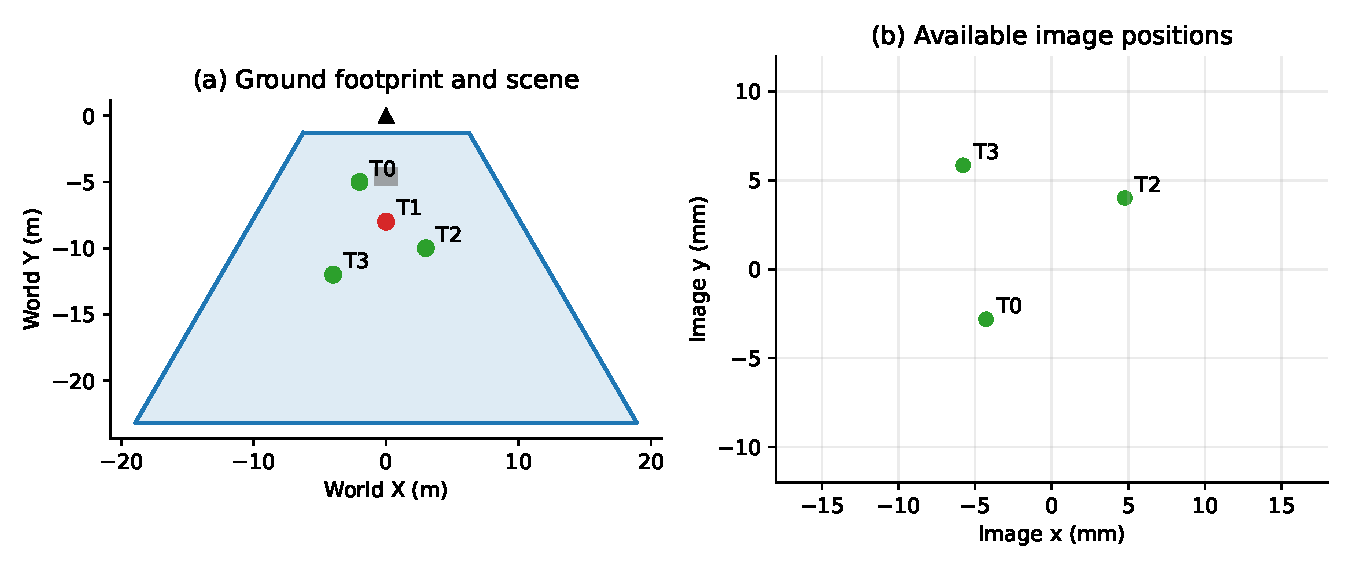
\includegraphics[width=.92\textwidth]{scene.pdf}
\caption{Baseline scene and sensor output. Green ground markers are visible; the red target is occluded. The obstacle is gray. Image coordinates are shown in millimeters.}
\label{fig:scene}
\end{figure}

Figure~\ref{fig:height} compares the independently calculated footprint area and target projection with Eq.~\eqref{eq:height}. Coverage increases from \HeightAreaMin{} to \HeightAreaMax{} m$^2$ as height increases from 4 to 12 m. The maximum relative area discrepancy is $\HeightAreaError$, consistent with floating-point roundoff. The target's image displacement decreases from 5 to approximately 1.667 mm. Greater coverage therefore accompanies reduced projected spatial scale; this is a geometric tradeoff, not a measured detection-resolution limit.
\begin{figure}[htbp]
\centering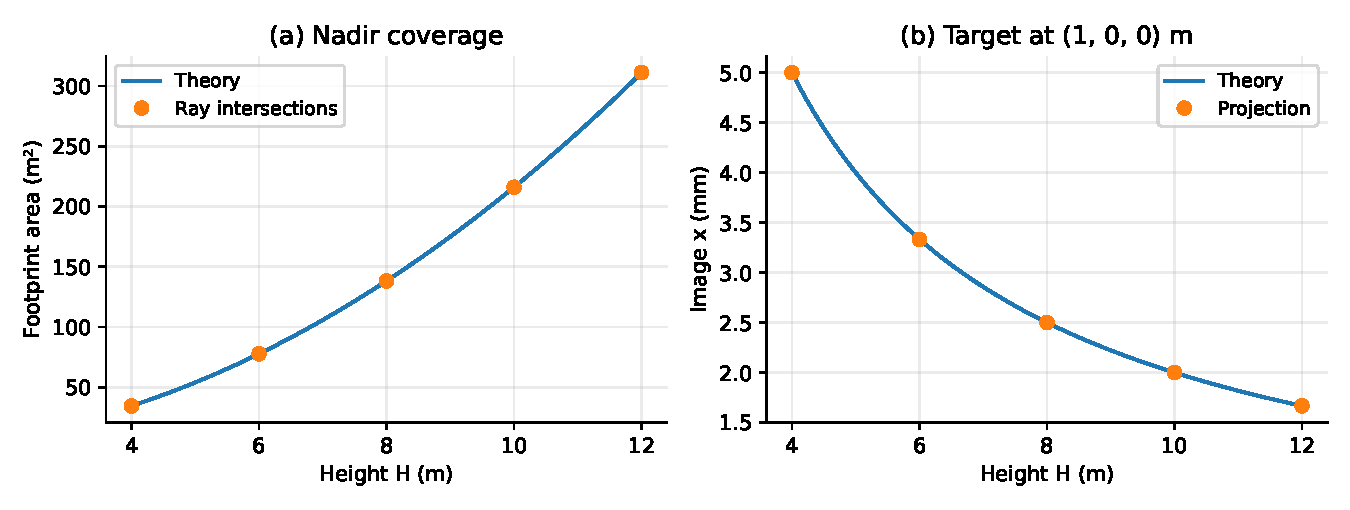
\includegraphics[width=.92\textwidth]{height.pdf}
\caption{Height-only experiment: analytic predictions and independently computed geometry agree. The camera is vertical and the target is fixed at $(1,0,0)$ m.}
\label{fig:height}
\end{figure}

\subsection{Orientation}
The pan sweep changes the number of available targets from one to three (Fig.~\ref{fig:orientation}a). Its maximum relative area change is $\PanAreaError$, confirming area invariance within numerical precision. Pan changes FOV selection but cannot change the LOS geometry of a fixed target when the camera center and obstacles are fixed.

Tilt has a different effect: footprint area decreases from \TiltAreaFirst{} to \TiltAreaLast{} m$^2$ between $125^\circ$ and $175^\circ$. The large low-tilt area is caused by corner rays approaching the horizon. All tested corners still intersect the ground forward, but no finite range limit is modeled. For the fixed target $(0,-8,0)$, Eq.~\eqref{eq:tilt} predicts the image-edge crossing at approximately $165.964^\circ$. The last visible sampled angle is $165^\circ$, and the first unavailable angle is $166^\circ$, matching the $1^\circ$ sampling resolution.
\begin{figure}[htbp]
\centering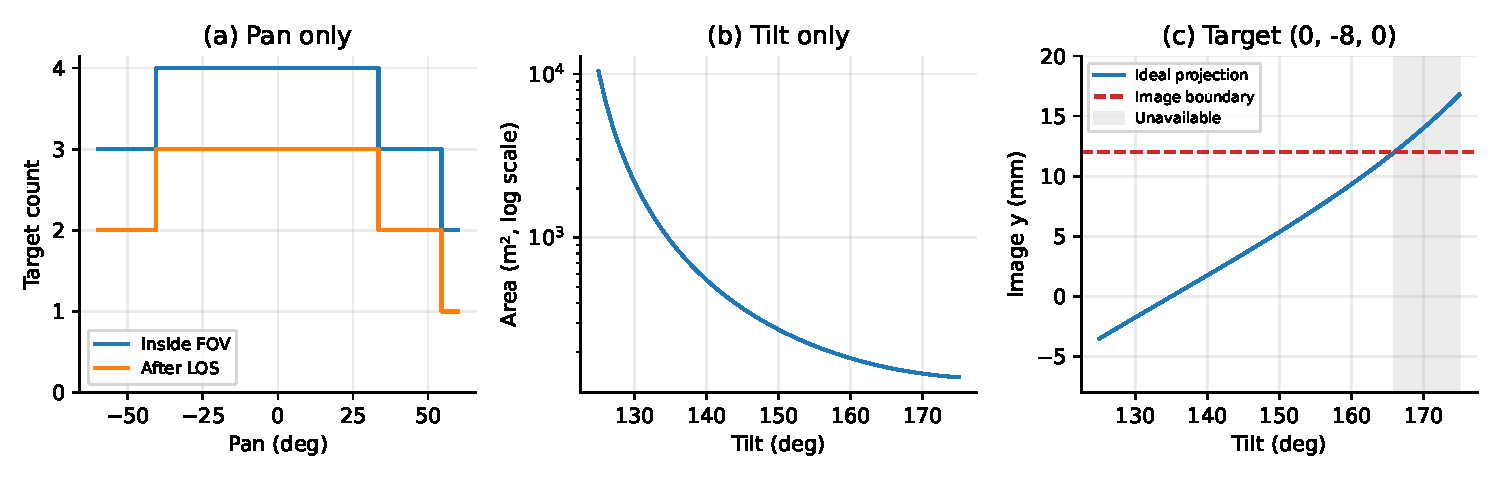
\includegraphics[width=\textwidth]{orientation.pdf}
\caption{Independent orientation experiments. Panel (a) changes pan with the static scene fixed. Panels (b)--(c) change tilt with no obstacle. The dashed line is the image boundary; gray shading indicates unavailable observations.}
\label{fig:orientation}
\end{figure}

\subsection{Target motion and environmental change}
For the target-only trajectory, depth is constant at $q_z=8(\sin140^\circ-\cos140^\circ)$ m. The horizontal FOV boundary occurs at $|x|=a q_z/(2f)$, giving analytic entry and exit times of \EntryTime{} and \ExitTime{} s. The simulation yields \VisibleSamples{} visible samples out of \MotionSamples{}, with first and last visible samples at \FirstSampleTime{} and \LastSampleTime{} s. Every sampled visibility classification agrees with the analytic interval. The image displacement is linear in time, with predicted slope \ImageSpeed{} mm/s (Fig.~\ref{fig:motion}a--b). Temporal quantization explains why sampled transition times do not equal the continuous-time crossings.

For the obstacle-height experiment, the sight line from $(0,0,8)$ to $(0,-8,0)$ satisfies $z=8+y$. Its minimum height over the obstacle's horizontal extent occurs at $y=-5.2$, giving a critical box height of \CriticalHeight{} m. The target is visible below this height and blocked at or above it because grazing contact is included. All 51 tested heights match that prediction (Fig.~\ref{fig:motion}c--d). This experiment changes the environment independently of the camera and target.
\begin{figure}[htbp]
\centering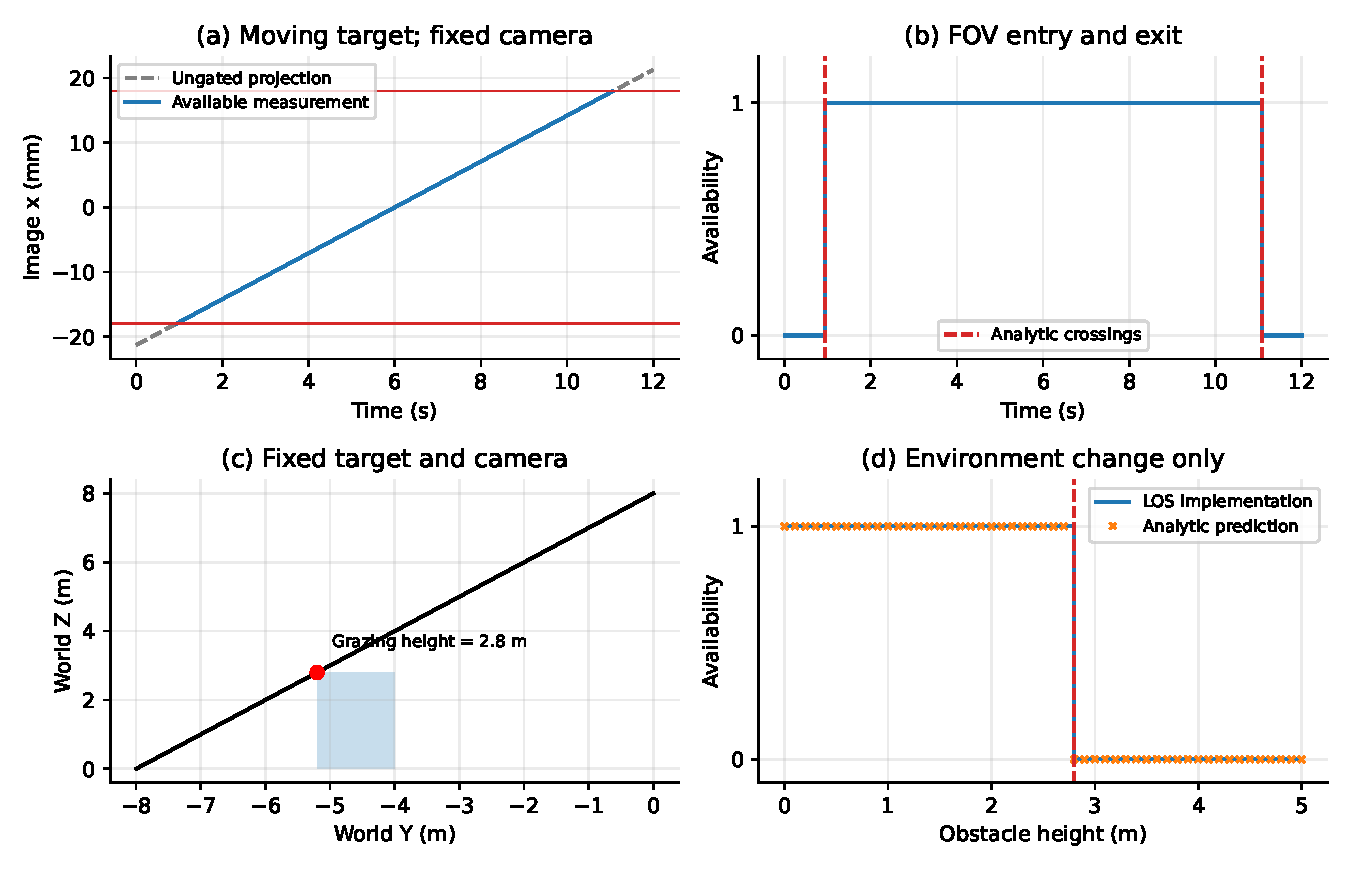
\includegraphics[width=.94\textwidth]{motion_occlusion.pdf}
\caption{Independent target and environment experiments. Missing measurements are omitted from the solid position curve. Analytic crossing times and the grazing-height threshold explain the observed availability transitions.}
\label{fig:motion}
\end{figure}

\subsection{Noise, sensitivity, and limits}
Table~\ref{tab:validation} summarizes the numerical checks. At $\sigma=0.5$ mm, the observed radial RMSE is \NoiseMaxRMSE{} mm, compared with approximately 0.707107 mm predicted. Finite-sample agreement supports the assumed random-noise implementation, not a real-camera noise law.
\begin{table}[htbp]
\centering\small
\caption{Numerical verification results for the selected conditions.}
\label{tab:validation}
\begin{tabular}{ll}\toprule
Comparison & Result\\\midrule
Height area: maximum relative discrepancy & $\HeightAreaError$\\
Pan area: maximum relative change & $\PanAreaError$\\
Target visibility: mismatched samples & $0/601$\\
Obstacle visibility: mismatched heights & $0/51$\\
Noise RMS: maximum relative discrepancy & $\NoisePercentError\%$\\
Projection derivative: error at $\delta=10^{-5}$ m & $\JacobianLast$ m/m\\\bottomrule
\end{tabular}
\end{table}

The maximum Jacobian component discrepancy decreases from $\JacobianFirst$ at $\delta=10^{-2}$ m to $\JacobianLast$ at $\delta=10^{-5}$ m (Fig.~\ref{fig:validation}). Agreement supports the implemented local derivative on the selected positive-depth points. Visibility gates and optical singularities are excluded from this local comparison.
\begin{figure}[htbp]
\centering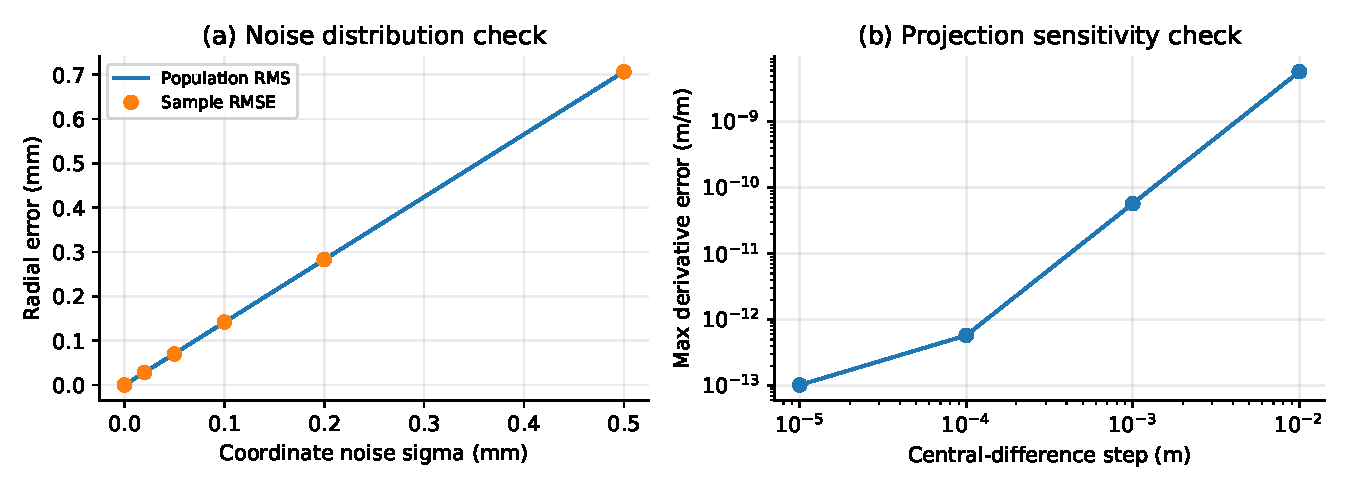
\includegraphics[width=.92\textwidth]{validation.pdf}
\caption{Separate checks of noise statistics and projection sensitivity. Panel (a) uses 10,000 samples per condition. Panel (b) compares analytic derivatives with central differences over three test points.}
\label{fig:validation}
\end{figure}

The animation and its 240 target-frame records visualize simultaneous changes, while the controlled experiments establish individual dependencies. Remaining errors or discrepancies arise from floating-point arithmetic, finite temporal/angular steps, central-difference approximation and finite Monte Carlo sampling. More substantial limitations are structural: point targets, a perfectly flat ground plane, ideal optics, opaque boxes, and prescribed camera motion. No lens distortion, image detector, motor response, physical maximum range or independently acquired real-image data is modeled. Consequently the results support synthetic consistency within these assumptions, not physical calibration or closed-loop tracking performance.

\section{Conclusions}
The project implements a PT camera position sensor and verifies its dependence on camera height, orientation, target motion, and environmental occlusion using controlled experiments. Coverage follows the predicted quadratic height law; pan preserves footprint area while changing target selection; tilt changes coverage and projection; and analytic visibility thresholds explain the sampled target and obstacle experiments. The noise and derivative checks support the chosen stochastic model and local sensitivity calculation. A reproducible configuration, numerical data and synchronized three-dimensional media connect the mathematical model to its simulated behavior. Future work should prioritize independent camera calibration and landmark reprojection measurements if physical accuracy is required; image-velocity sensing or actuator control can then be added for tasks that specifically need them.

\begin{thebibliography}{9}
\bibitem{assignment} S. Ferrari, ``Midterm project,'' Robot Perception, CEE/MAE 4810/5810 and ECE 4240/5240, course assignment, n.d.
\bibitem{handout} S. Ferrari, ``Pinhole camera model and field-of-view (FOV),'' MAE 4810/5810 Robot Perception, course handout, n.d.
\bibitem{writing} S. Ferrari, ``Writing guidelines,'' Robot Perception, course handout, Oct. 2, 2023.
\end{thebibliography}
\end{document}
